\documentclass[12pt]{article}
\usepackage[utf8]{inputenc}
\usepackage[ukrainian]{babel}
\usepackage{graphicx}
\usepackage[a6paper, landscape, margin=0.8cm]{geometry}
\usepackage{multicol}


\pagestyle{empty} % прибирає нумерацію


\begin{document}


\begin{minipage}{\linewidth}


\begin{multicols}{2}


% --- ЛІВА КОЛОНКА (ФОТО) ---
\begin{center}
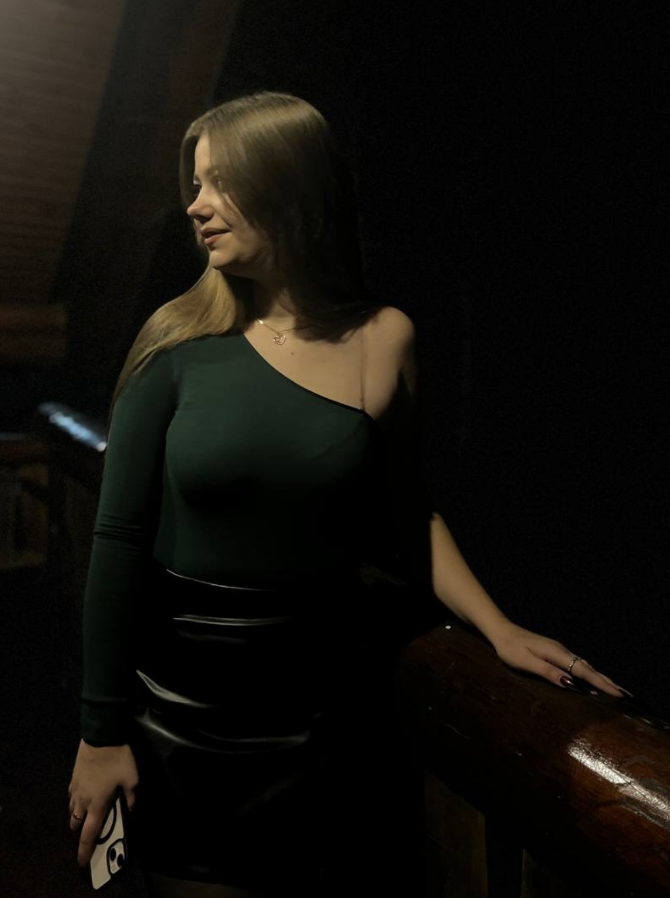
\includegraphics[width=0.8\linewidth]{foto.png}
\end{center}


\columnbreak


% --- ПРАВА КОЛОНКА (ІНФОРМАЦІЯ) ---
\textbf{\Large Валерія}


\vspace{0.3cm}


\textit{Студент / Репетитор}


\vspace{0.5cm}


lera1golovata@gmail.com


+380 96 128 23 69


\vspace{0.5cm}


\textbf{займаюсь з дітьми 1-5 класу:}


\begin{itemize}
\item навчу рахувати
\item доженемо програму зі школи
\item заохочу любити математику
\end{itemize}


\vspace{0.5cm}


\textit{зі мною математика стає простою, граємо в ігри та вивчаємо}




\end{multicols}


\end{minipage}


\end{document}

